\documentclass[aspectratio=169,11pt]{beamer}

\usepackage[T1]{fontenc}
\usepackage{lmodern}
\usepackage{amsmath,amssymb}
\usepackage{booktabs}
\usepackage{graphicx}
\usepackage{xcolor}
\usepackage{listings}

\definecolor{courseblue}{RGB}{0,91,155}
\definecolor{courseorange}{RGB}{190,72,20}
\definecolor{codebg}{RGB}{247,248,250}
\definecolor{codeframe}{RGB}{210,216,224}
\definecolor{codecomment}{RGB}{78,128,88}
\definecolor{codestring}{RGB}{160,72,30}
\definecolor{codekeyword}{RGB}{0,91,155}

\setbeamercolor{structure}{fg=courseblue}
\setbeamercolor{frametitle}{fg=courseblue}
\setbeamercolor{alerted text}{fg=courseorange}
\setbeamertemplate{navigation symbols}{}
\setbeamertemplate{footline}[frame number]
\setbeamertemplate{itemize items}[circle]
\setbeamertemplate{enumerate items}[default]

\lstdefinestyle{matlabcode}{
  language=Matlab,
  basicstyle=\ttfamily\tiny,
  keywordstyle=\bfseries\color{codekeyword},
  commentstyle=\itshape\color{codecomment},
  stringstyle=\color{codestring},
  backgroundcolor=\color{codebg},
  frame=single,
  rulecolor=\color{codeframe},
  framerule=0.5pt,
  numbers=left,
  numberstyle=\tiny\color{gray},
  xleftmargin=1.5em,
  framexleftmargin=1.2em,
  breaklines=true,
  columns=fullflexible,
  keepspaces=true,
  showstringspaces=false,
  tabsize=4
}
\lstset{style=matlabcode}

\newcommand{\codefile}[1]{\texttt{#1}}
\newcommand{\takeaway}[1]{%
  \vspace{0.3em}
  \begin{beamercolorbox}[rounded=true,sep=0.7em,wd=\linewidth]{block body}
    \textbf{Takeaway.} #1
  \end{beamercolorbox}
}

\title{Reading the MATLAB Code for Elliptical Slice Sampling}
\subtitle{\codefile{demo\_ess.m} and \codefile{elliptical\_slice\_step.m}}
\author{Econometrics 32706}
\date{}

\begin{document}

\begin{frame}{Model and Posterior Used in the Demo}
  {\footnotesize Source files: \codefile{demo\_ess.m} and \codefile{elliptical\_slice\_step.m}}\par
  \vspace{0.25em}

  \begin{block}{Model in the code}
  \[
    f \sim \mathcal N(0,K),\qquad
    K=\begin{pmatrix}1&0.8\\0.8&1\end{pmatrix}
  \]
  \[
    y = h f + \varepsilon,\qquad
    h=(1,0),\qquad
    \varepsilon\sim\mathcal N(0,\sigma^2),\qquad
    y=1,\quad \sigma=0.35.
  \]
  \end{block}

  \begin{block}{Posterior target}
  \[
    p(f\mid y) \propto L(f)\,\mathcal N(f;0,K),
    \qquad
    \log L(f)=-\frac{1}{2}\frac{(y-hf)^2}{\sigma^2}.
  \]
  \[
    f\mid y\sim\mathcal N(m,C),\qquad
    \begin{aligned}
      m &= Kh'(hKh'+\sigma^2)^{-1}y,\\
      C &= K-Kh'(hKh'+\sigma^2)^{-1}hK.
    \end{aligned}
  \]
  \end{block}
\end{frame}

\begin{frame}{What the code does}
  \begin{columns}[T,totalwidth=\textwidth]
    \begin{column}{0.52\textwidth}
      \begin{itemize}
        \setlength{\itemsep}{0.75em}
        \item \codefile{demo\_ess.m} builds a two-variable Gaussian example.
        \item \codefile{elliptical\_slice\_step.m} performs one Markov chain update.
        \item The demo checks the sampler against the exact Gaussian posterior.
        \item The final plot compares simulated draws, the exact posterior contour, and the prior contour.
      \end{itemize}
    \end{column}
    \begin{column}{0.43\textwidth}
      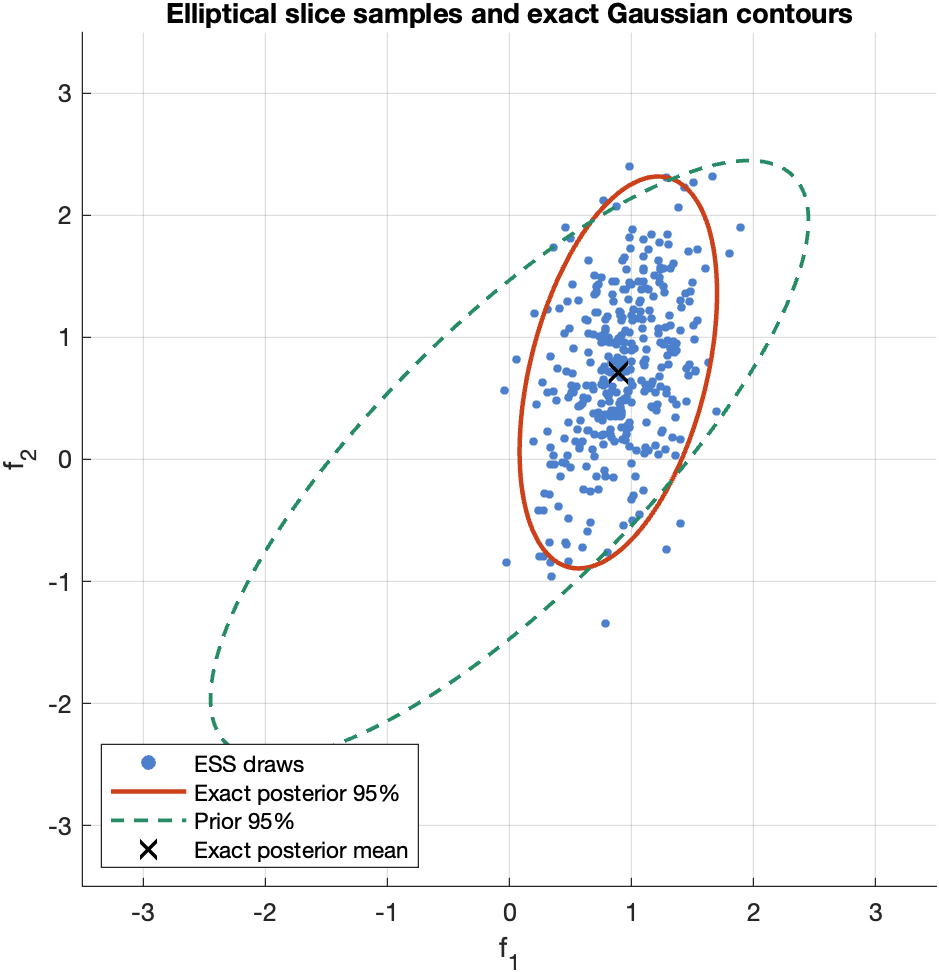
\includegraphics[width=\linewidth,height=0.62\textheight,keepaspectratio]{ess_demo.png}
    \end{column}
  \end{columns}
  \takeaway{The demo is small because all model-specific information enters through a covariance matrix and a log-likelihood function.}
\end{frame}

\begin{frame}[fragile]{Step 1: reset and define the model}
  \begin{columns}[T,totalwidth=\textwidth]
    \begin{column}{0.58\textwidth}
      \lstinputlisting[firstline=1,lastline=14]{demo_ess.m}
    \end{column}
    \begin{column}{0.37\textwidth}
      \begin{itemize}
        \setlength{\itemsep}{0.7em}
        \item \texttt{rng(32706)} makes the simulation reproducible.
        \item \(K\) is the prior covariance of \(f=(f_1,f_2)'\).
        \item The observation is \(y=f_1+\varepsilon\), with \(\varepsilon\sim N(0,\sigma^2)\).
        \item \texttt{loglike} is the only likelihood object the ESS update needs.
      \end{itemize}
    \end{column}
  \end{columns}
\end{frame}

\begin{frame}[fragile]{Step 2: compute the exact posterior}
  \begin{columns}[T,totalwidth=\textwidth]
    \begin{column}{0.56\textwidth}
      \lstinputlisting[firstline=16,lastline=19]{demo_ess.m}
    \end{column}
    \begin{column}{0.39\textwidth}
      The example is deliberately linear-Gaussian, so the posterior is available in closed form:
      \[
        \begin{aligned}
          C &= K - K h'(hKh' + \sigma^2)^{-1}hK,\\
          m &= K h'(hKh' + \sigma^2)^{-1}y.
        \end{aligned}
      \]
      These exact moments are not needed by the sampler. They are used to verify the code.
    \end{column}
  \end{columns}
  \takeaway{The exact posterior is a benchmark for the lesson, not an input to ESS.}
\end{frame}

\begin{frame}[fragile]{Step 3: run the Markov chain}
  \begin{columns}[T,totalwidth=\textwidth]
    \begin{column}{0.58\textwidth}
      \lstinputlisting[firstline=21,lastline=34]{demo_ess.m}
    \end{column}
    \begin{column}{0.37\textwidth}
      \begin{enumerate}
        \setlength{\itemsep}{0.65em}
        \item Start the chain at \(f=(0,0)'\).
        \item Run \texttt{nBurn + nKeep} updates.
        \item Store only draws after burn-in.
        \item Count likelihood evaluations to measure computational effort.
      \end{enumerate}
    \end{column}
  \end{columns}
\end{frame}

\begin{frame}[fragile]{Step 4: compare exact and simulated moments}
  \begin{columns}[T,totalwidth=\textwidth]
    \begin{column}{0.57\textwidth}
      \lstinputlisting[firstline=36,lastline=44]{demo_ess.m}
    \end{column}
    \begin{column}{0.38\textwidth}
      \begin{itemize}
        \setlength{\itemsep}{0.75em}
        \item The posterior mean is estimated by the average of stored draws.
        \item The posterior covariance is estimated with \texttt{cov(samples')}.
        \item The printed output lets students check convergence numerically before looking at the plot.
      \end{itemize}
    \end{column}
  \end{columns}
\end{frame}

\begin{frame}[fragile]{Step 5: prepare posterior and prior contours}
  \begin{columns}[T,totalwidth=\textwidth]
    \begin{column}{0.6\textwidth}
      \lstinputlisting[firstline=46,lastline=53]{demo_ess.m}
    \end{column}
    \begin{column}{0.35\textwidth}
      {\footnotesize
      \[
        \begin{aligned}
          d^2_p(f) &= (f-m)'C^{-1}(f-m),\\
          d^2_0(f) &= f'K^{-1}f.
        \end{aligned}
      \]
      }
      The value \(5.991\) is the 95 percent quantile of a chi-square distribution with two degrees of freedom.
    \end{column}
  \end{columns}
\end{frame}

\begin{frame}[fragile]{Step 6a: draw the figure}
  \begin{columns}[T,totalwidth=\textwidth]
    \begin{column}{0.6\textwidth}
      \lstinputlisting[firstline=55,lastline=66]{demo_ess.m}
    \end{column}
    \begin{column}{0.35\textwidth}
      \begin{itemize}
        \setlength{\itemsep}{0.7em}
        \item A subset of draws is shown to avoid overplotting.
        \item The posterior contour is solid orange.
        \item The prior contour is green and dashed.
        \item The exact posterior mean is marked with a black cross.
        \item \texttt{exportgraphics} writes \codefile{ess\_demo.png}.
      \end{itemize}
    \end{column}
  \end{columns}
\end{frame}

\begin{frame}[fragile]{Step 6b: label and export the figure}
  \begin{columns}[T,totalwidth=\textwidth]
    \begin{column}{0.6\textwidth}
      \lstinputlisting[firstline=67,lastline=75]{demo_ess.m}
    \end{column}
    \begin{column}{0.35\textwidth}
      \begin{itemize}
        \setlength{\itemsep}{0.7em}
        \item The exact posterior mean is marked with a black cross.
        \item The legend identifies the draws, prior, posterior, and mean.
        \item \texttt{exportgraphics} writes \codefile{ess\_demo.png}.
      \end{itemize}
    \end{column}
  \end{columns}
\end{frame}

\begin{frame}{The resulting picture}
  \centering
  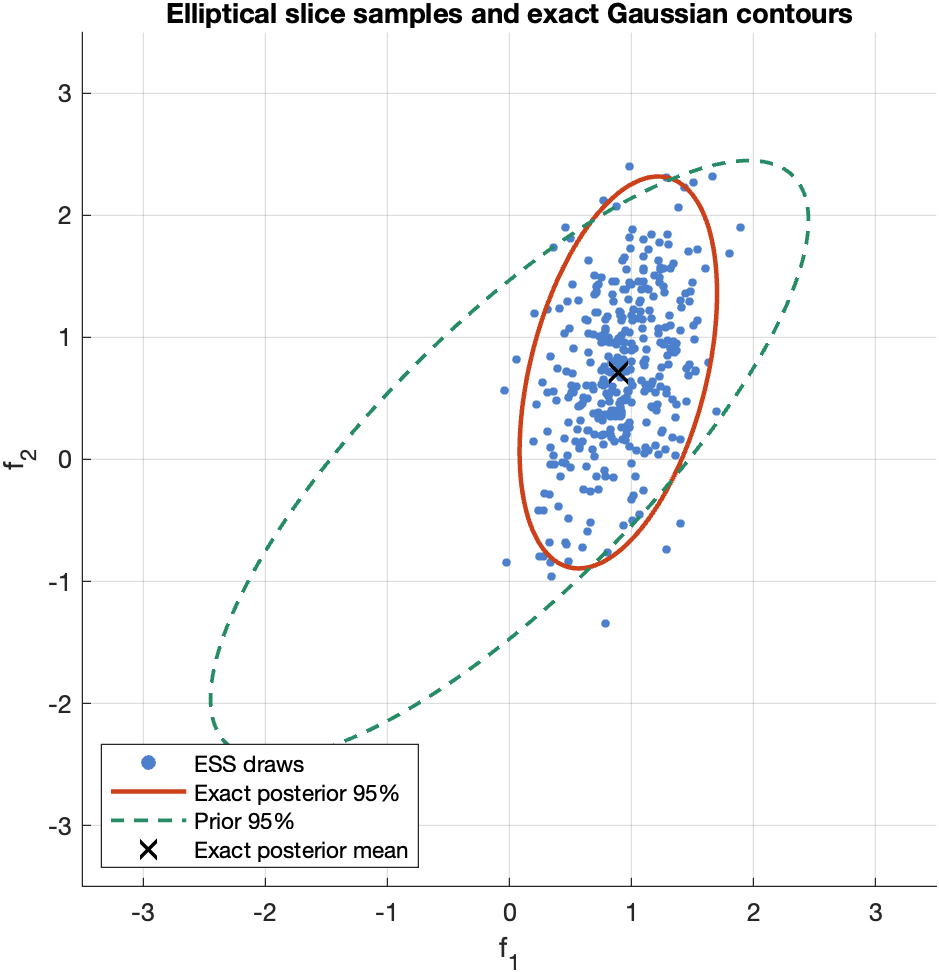
\includegraphics[width=0.9\textwidth,height=0.82\textheight,keepaspectratio]{ess_demo.png}
\end{frame}

\begin{frame}[fragile]{Inside one ESS update: input checks}
  \begin{columns}[T,totalwidth=\textwidth]
    \begin{column}{0.58\textwidth}
      \lstinputlisting[firstline=1,lastline=21]{elliptical_slice_step.m}
    \end{column}
    \begin{column}{0.37\textwidth}
      \begin{itemize}
        \setlength{\itemsep}{0.7em}
        \item The state is forced into a column vector.
        \item \texttt{cholK} must be an \(n\times n\) lower Cholesky factor.
        \item The current log-likelihood must be finite and scalar.
        \item \texttt{nEval} starts at one because the current state is evaluated once.
      \end{itemize}
    \end{column}
  \end{columns}
\end{frame}

\begin{frame}[fragile]{Inside one ESS update: slice and ellipse}
  \begin{columns}[T,totalwidth=\textwidth]
    \begin{column}{0.58\textwidth}
      \lstinputlisting[firstline=23,lastline=30]{elliptical_slice_step.m}
    \end{column}
    \begin{column}{0.37\textwidth}
      \begin{itemize}
        \setlength{\itemsep}{0.75em}
        \item \(\nu=\texttt{cholK}z\), with \(z\sim N(0,I)\), is an independent prior draw.
        \item The log slice level is below the current log-likelihood.
        \item The first angle is random on \([0,2\pi]\).
        \item The initial bracket has width \(2\pi\) and contains angle zero.
      \end{itemize}
    \end{column}
  \end{columns}
\end{frame}

\begin{frame}[fragile]{Inside one ESS update: propose and accept}
  \begin{columns}[T,totalwidth=\textwidth]
    \begin{column}{0.58\textwidth}
      \lstinputlisting[firstline=32,lastline=43]{elliptical_slice_step.m}
    \end{column}
    \begin{column}{0.37\textwidth}
      \begin{enumerate}
        \setlength{\itemsep}{0.6em}
        \item Propose \(f(\theta)=f\cos\theta+\nu\sin\theta\).
        \item Accept if the proposal is above the slice level.
        \item Return immediately once an acceptable point is found.
      \end{enumerate}
    \end{column}
  \end{columns}
\end{frame}

\begin{frame}[fragile]{Inside one ESS update: shrink and retry}
  \begin{columns}[T,totalwidth=\textwidth]
    \begin{column}{0.58\textwidth}
      \lstinputlisting[firstline=45,lastline=53]{elliptical_slice_step.m}
    \end{column}
    \begin{column}{0.37\textwidth}
      \begin{enumerate}
        \setlength{\itemsep}{0.65em}
        \item A rejected angle cuts away one side of the bracket.
        \item Angle zero remains in the bracket, so the current state is always available.
        \item The loop draws from the smaller bracket until it finds an angle above the slice.
      \end{enumerate}
    \end{column}
  \end{columns}
\end{frame}

\begin{frame}{Why this update is convenient}
  \begin{itemize}
    \setlength{\itemsep}{0.9em}
    \item It uses the Gaussian prior geometry instead of a random-walk proposal.
    \item It requires no proposal variance or step-size tuning.
    \item The likelihood can be swapped by changing only the \texttt{loglike} function handle.
    \item The accepted point is always on the prior ellipse through the current state and an independent prior draw.
  \end{itemize}
  \takeaway{The sampler separates prior geometry from likelihood evaluation, which is why the implementation is compact.}
\end{frame}

    \scriptsize
\begin{frame}{Files produced by the demo}
  \begin{center}
    \begin{tabular}{@{}lll@{}}
      \toprule
      File & Role & Key idea\\
      \midrule
      \codefile{demo\_ess.m} & driver script & define model, run chain, plot checks\\
      \codefile{elliptical\_slice\_step.m} & sampler step & slice level plus angular bracket shrinking\\
      \codefile{ess\_demo.png} & output figure & simulated draws vs exact contours\\
      \codefile{beamer.tex} & lecture deck & step-by-step code walkthrough\\
      \bottomrule
    \end{tabular}
  \end{center}
\end{frame}

\end{document}
